\documentclass[runningheads]{llncs}

\usepackage[T1]{fontenc}
\usepackage[utf8]{inputenc}
\usepackage{graphicx}
\usepackage{booktabs}
\usepackage{multirow}
\usepackage{amsmath}
\usepackage{amssymb}
\usepackage[section]{placeins}
\usepackage{tikz}
\usetikzlibrary{arrows.meta,positioning,fit}
\usepackage{url}

\begin{document}

\title{XBone-Net: Parameter-Efficient Multimodal Fusion of Musculoskeletal Radiographs and Clinical History with Reliability Auditing}
\titlerunning{XBone-Net for Multimodal Musculoskeletal Radiograph Classification}

\author{Nguyen Van Le Ba Thanh\inst{1} \and
Nguyen Gia Kiet\inst{1} \and
Ly Quoc Ngoc\inst{1} \and
Do Thi Thanh Ha\inst{1}}
\authorrunning{N. V. L. B. Thanh et al.}

\institute{Faculty of Information Technology, University of Science, Vietnam National University Ho Chi Minh City, Ho Chi Minh City, Vietnam}

\maketitle

\begin{abstract}
Musculoskeletal radiograph classification is challenging when labeled data are limited, class frequencies are highly imbalanced, and visually similar conditions require contextual clinical information. We present XBone-Net, a parameter-efficient multimodal framework that combines a radiograph with its associated clinical history. The method adapts the image and text encoders of BiomedCLIP using low-rank adaptation (LoRA), preserves both a global radiograph view and four automatically selected high-detail local views, aligns image and text representations through a semantic matching stage, and learns bidirectional cross-attention followed by an empirical class-centroid classifier. We further audit the learned representation using post-hoc Mahalanobis out-of-distribution (OOD) scores, input interventions, and Integrated Gradients. Experiments use three random seeds on CTCH, a private patient-disjoint dataset containing 3,249 radiograph-history pairs from 22 musculoskeletal classes, and BTXRD, a public 10-class bone-tumor dataset containing 3,746 radiographs with metadata-derived text. On CTCH, XBone-Net obtains a Macro-F1 of $0.5558\pm0.0072$, Macro-AUROC of $0.9473\pm0.0246$, and Macro-AUPRC of $0.6189\pm0.0145$ while updating 8.63M parameters, or 4.22\% of the model. Paired image-history input improves Macro-F1 by 0.1574 over image-only input, whereas cross-class history replacement reduces it to $0.3039\pm0.0048$. Mahalanobis scoring detects near-domain semantic OOD with AUROC $0.6286\pm0.0177$ and cross-dataset shift with AUROC $0.8042\pm0.0938$, but high FPR at 95\% TPR prevents automatic rejection. The results show that clinical history provides useful complementary signal and that parameter efficiency does not imply computational efficiency. XBone-Net is therefore positioned as a reproducible multimodal classification and reliability-auditing framework rather than a clinically validated diagnostic system.

\keywords{Multimodal learning \and Musculoskeletal radiographs \and Vision-language models \and Parameter-efficient fine-tuning \and Out-of-distribution detection \and Explainable artificial intelligence}
\end{abstract}

\section{Introduction}

Radiographs are among the most common medical images, yet automated musculoskeletal interpretation remains difficult. Fractures and bone lesions may be small relative to the field of view, multiple anatomical regions must be handled by one model, and clinically important classes can be severely under-represented. In routine care, an image is not interpreted in isolation: the injury mechanism, pain location, disease course, and medical history influence the diagnostic hypothesis. Models that ignore this information discard a source of context already available at the point of interpretation.

Vision-language pretraining offers a natural starting point for this setting. CLIP-style learning aligns images and text in a shared space \cite{CLIP}, while medical variants learn from radiographs and reports \cite{ConVIRT,GLoRIA,MedCLIP,BiomedCLIP}. However, directly transferring these models to small musculoskeletal datasets leaves three practical gaps. First, a fixed square input can suppress fine structures when a long radiograph is globally resized. Second, full fine-tuning is expensive and may overfit limited labeled data. Third, a competitive classification score alone does not characterize behavior under inconsistent text, distribution shift, or explanation perturbations.

We address these gaps with XBone-Net, a two-stage multimodal framework built on BiomedCLIP \cite{BiomedCLIP}. A radiograph is represented by one global view and four deterministic, label-free local crops. LoRA adapters \cite{Hu2022LoRA} update the image and text encoders while the pretrained backbone remains frozen. A semantic matching stage first adapts the two modalities to the target domain. Bidirectional cross-attention then exchanges image and clinical context, and a class-centroid head performs supervised classification. The fused representation is additionally evaluated using post-hoc OOD scores and attribution interventions.

The paper makes four contributions:
\begin{enumerate}
    \item We propose a parameter-efficient musculoskeletal vision-language architecture that preserves global anatomy and local detail without requiring lesion annotations.
    \item We formulate a two-stage training procedure combining soft semantic image-text matching with class-balanced centroid classification.
    \item We evaluate modality dependence, component alternatives, parameter and inference costs, near-domain and cross-dataset OOD detection, and attribution faithfulness under a common three-seed protocol.
    \item We provide a calibrated empirical account: multimodal input is beneficial on the primary clinical dataset, but the complete architecture is not a universal winner, OOD false-positive rates remain high, and the explanations do not establish lesion localization or clinical validity.
\end{enumerate}

The intended contribution is consequently methodological and evaluative. This study does not claim state-of-the-art performance or readiness for clinical deployment.

\section{Related Work}

\subsection{Medical Vision-Language Learning}

General-domain CLIP learns transferable visual concepts through large-scale image-text contrastive training \cite{CLIP}. Medical approaches exploit naturally paired images and reports. ConVIRT applies bidirectional contrastive learning to paired medical data \cite{ConVIRT}; GLoRIA combines global and local image-text alignment \cite{GLoRIA}; and MedCLIP introduces semantic matching to reduce false negatives caused by clinically similar reports from different patients \cite{MedCLIP}. BiomedCLIP scales biomedical pretraining to 15 million image-text pairs and couples a Vision Transformer image encoder with a biomedical text encoder \cite{BiomedCLIP}. XBone-Net uses BiomedCLIP as a frozen foundation and adapts it to musculoskeletal classification. In contrast to pretraining work, our focus is a constrained downstream setting with patient history, severe class imbalance, local high-resolution views, and explicit reliability audits.

\subsection{Parameter-Efficient and Metric-Based Adaptation}

LoRA represents a weight update as the product of two low-rank matrices, reducing the number of optimized parameters while preserving the pretrained weights \cite{Hu2022LoRA}. We apply LoRA to linear layers in both the vision and language encoders. The final classifier is inspired by prototypical networks, which represent each class by the mean of its support embeddings \cite{Snell2017ProtoNet}. Class centroids provide an interpretable geometry and a shared representation for classification and post-hoc distance scoring. Because rare musculoskeletal classes contain few samples, we combine this head with effective-number class weights \cite{Cui2019ClassBalanced}.

\subsection{Reliability Beyond Classification}

Maximum softmax probability is a standard baseline for detecting anomalous predictions \cite{Hendrycks2017MSP}. Feature-distance approaches instead quantify separation from the training representation; Mahalanobis distance is a simple and competitive example \cite{Lee2018MahalanobisOOD}, while deep nearest-neighbor distance offers a non-parametric alternative \cite{Sun2022KNN}. We use these methods only as post-hoc warnings, not as evidence of safe rejection. For explanation, Integrated Gradients attributes the change from a baseline input to the observed prediction \cite{Sundararajan2017IntegratedGradients}. Attribution maps can nevertheless look plausible without being faithful, so we accompany qualitative examples with source replacement and deletion/insertion controls.

\section{Method}

\subsection{Problem Formulation and Overview}

Let $\mathcal{D}=\{(x_i^{I},x_i^{T},y_i)\}_{i=1}^{N}$ contain a radiograph $x_i^{I}$, associated clinical text $x_i^{T}$, and a single class $y_i\in\{1,\ldots,K\}$. XBone-Net maps each pair to a fused representation $z_i\in\mathbb{R}^{512}$ and estimates class probabilities $p(y=k\mid z_i)$. Figure~\ref{fig:architecture} summarizes the pipeline.

\begin{figure}[t]
\centering
\resizebox{\textwidth}{!}{%
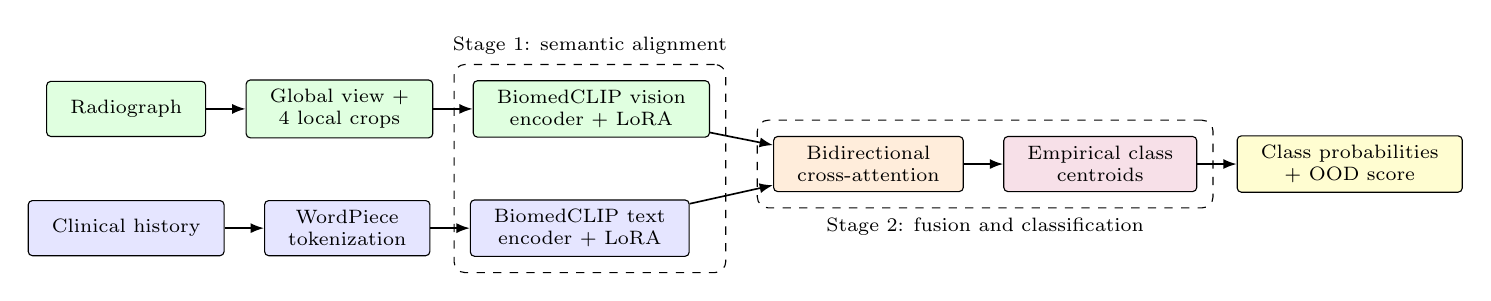
\begin{tikzpicture}[
    font=\scriptsize,
    node distance=3.5mm and 5mm,
    box/.style={draw, rounded corners=1.5pt, align=center, minimum height=7mm, inner xsep=3mm},
    arrow/.style={-{Latex[length=1.7mm]}, semithick}
]
\node[box, fill=green!12] (img) {Radiograph};
\node[box, fill=green!12, right=of img] (views) {Global view +\\4 local crops};
\node[box, fill=green!12, right=of views] (ve) {BiomedCLIP vision\\encoder + LoRA};

\node[box, fill=blue!10, below=8mm of img] (text) {Clinical history};
\node[box, fill=blue!10, right=of text] (tok) {WordPiece\\tokenization};
\node[box, fill=blue!10, right=of tok] (te) {BiomedCLIP text\\encoder + LoRA};

\node[box, fill=orange!14, right=8mm of ve, yshift=-7mm] (fusion) {Bidirectional\\cross-attention};
\node[box, fill=purple!12, right=of fusion] (centroid) {Empirical class\\centroids};
\node[box, fill=yellow!18, right=of centroid] (out) {Class probabilities\\+ OOD score};

\draw[arrow] (img) -- (views);
\draw[arrow] (views) -- (ve);
\draw[arrow] (text) -- (tok);
\draw[arrow] (tok) -- (te);
\draw[arrow] (ve) -- (fusion);
\draw[arrow] (te) -- (fusion);
\draw[arrow] (fusion) -- (centroid);
\draw[arrow] (centroid) -- (out);

\node[draw, dashed, rounded corners, fit=(ve)(te), inner sep=2mm, label={[font=\scriptsize]above:Stage 1: semantic alignment}] {};
\node[draw, dashed, rounded corners, fit=(fusion)(centroid), inner sep=2mm, label={[font=\scriptsize]below:Stage 2: fusion and classification}] {};
\end{tikzpicture}
}
\caption{XBone-Net. Stage 1 adapts frozen BiomedCLIP encoders through LoRA and soft image-text semantic matching. Stage 2 learns cross-attention and a class-centroid decision space. OOD scoring and explanation are post-hoc analyses.}
\label{fig:architecture}
\end{figure}

\subsection{Global and Sparse-Focal Image Representation}

BiomedCLIP receives $224\times224$ images. To retain overall anatomy and localized detail, we create one global view and four local crops from each radiograph. Crop selection uses only pixel values; labels, text, and lesion annotations are never consulted. We first estimate the border intensity and foreground mask, retain the content bounding box when it preserves at least 95\% of contrast energy, and otherwise fall back to the full image. The global content is aspect-ratio preserved, padded with the border median, and resized to $224\times224$.

For local views, the content image is scaled to a maximum long side of 896 pixels without upsampling. Candidate $224\times224$ windows use stride 168 and are scored using normalized Laplacian energy, grayscale entropy, and foreground ratio:
\begin{equation}
q(b)=0.55\widehat{E}(b)+0.35\widehat{H}(b)+0.10r(b).
\end{equation}
Two crops promote anatomical coverage and two promote high score with spatial diversity. Non-maximum suppression uses an intersection-over-union threshold of 0.30. This deterministic sparse-focal procedure always returns four crops.

The BiomedCLIP Vision Transformer \cite{Dosovitskiy2021ViT,BiomedCLIP} encodes the global image and four local views with shared weights. The global view contributes its class token $g_i$. Each local view retains its class token and a $2\times2$ adaptive average-pooled patch grid, producing five tokens. Coordinates are projected and added to the 20 local tokens. The resulting visual sequence is
\begin{equation}
V_i=[g_i;\tilde{\ell}_{i,1};\ldots;\tilde{\ell}_{i,20}]\in\mathbb{R}^{21\times512}.
\end{equation}

\subsection{Text Encoding and LoRA Adaptation}

Clinical history is tokenized with the BiomedCLIP text tokenizer, truncated or padded to the configured maximum length, and encoded into $H_i^T\in\mathbb{R}^{T\times512}$. For a frozen linear weight $W$, LoRA learns
\begin{equation}
W'=W+\frac{\alpha}{r}BA,
\quad A\in\mathbb{R}^{r\times d_i},\quad B\in\mathbb{R}^{d_o\times r},
\end{equation}
with rank $r=16$, scale $\alpha=32$, and dropout 0.1. Adapters are applied to attention and feed-forward projections in both encoders. All pretrained backbone weights remain fixed.

\subsection{Stage 1: Soft Semantic Matching}

Stage 1 aligns image and text representations in the target domain. Local tokens are attention-pooled and added to the global image vector with weight 0.25, yielding normalized image representation $\bar v_i$; the text class token yields $t_i$. For a batch of size $B$, similarity is $s_{ij}=\bar v_i^Tt_j/\tau$. Rather than treating every non-paired report as negative, the unnormalized target is 1 for the observed pair, $\rho=0.5$ for a different sample from the same class, and 0 for a different class. After row normalization in both image-to-text and text-to-image directions, the loss is
\begin{equation}
\mathcal{L}_{\mathrm{SM}}=-\frac{1}{2B}\sum_{i,j}
\left(q^{I\rightarrow T}_{ij}\log p^{I\rightarrow T}_{ij}
+q^{T\rightarrow I}_{ij}\log p^{T\rightarrow I}_{ij}\right).
\end{equation}
Class-aware sampling increases the chance of observing meaningful same-class pairs. The stage updates LoRA and local pooling parameters, but not the fusion or classifier.

\subsection{Stage 2: Bidirectional Fusion and Centroid Classification}

Stage 2 passes the visual and text sequences through independent linear projections and bidirectional cross-attention. The global image token queries non-padding text tokens, while the text class token queries the 20 local image tokens:
\begin{align}
h_i^{I\leftarrow T}&=\mathrm{LN}\left(\hat V_{i,0}+\mathrm{MHA}_{I\leftarrow T}(\hat V_{i,0:1},\hat H^T_{i,1:})_0\right),\\
h_i^{T\leftarrow I}&=\mathrm{LN}\left(\hat H^T_{i,0}+\mathrm{MHA}_{T\leftarrow I}(\hat H^T_{i,0:1},\hat V_{i,1:})_0\right).
\end{align}
An MLP fuses the two context-enriched vectors:
\begin{equation}
z_i=\mathrm{LN}\left(\mathrm{MLP}\left([h_i^{I\leftarrow T};h_i^{T\leftarrow I}]\right)\right).
\end{equation}

For class $k$, the empirical centroid is the mean training representation $c_k=|\mathcal{I}_k|^{-1}\sum_{i\in\mathcal{I}_k}z_i$. Cosine similarity is converted to a logit by $l_{ik}=\alpha_c\cos(z_i,c_k)+b_k$, where $b_k$ is a learned class bias. Centroids are recomputed from the training set before each validation pass and once more using the selected checkpoint. Weighted cross-entropy uses effective-number class weights, maximum relative weight 5.0, and label smoothing 0.05. Test samples never update model parameters or centroids.

\subsection{Post-hoc Reliability Auditing}

OOD detectors are fitted on training representations and calibrated only with in-distribution validation samples. The primary score is the minimum class-conditional Mahalanobis distance
\begin{equation}
s_{\mathrm{OOD}}(z)=\min_k\sqrt{(z-\mu_k)^T\Sigma^{-1}(z-\mu_k)},
\end{equation}
where a shared covariance $\Sigma$ is regularized by Ledoit-Wolf shrinkage \cite{LedoitWolf2004}. We compare centroid cosine distance, Mahalanobis distance, five-nearest-neighbor distance, and predictive entropy. Integrated Gradients is computed for global image, local image, and text inputs. Faithfulness is evaluated by deletion and insertion following attribution order and by a random-order control. These analyses quantify sensitivity to the selected baselines; they do not prove causal contribution or clinical correctness.

\section{Experimental Design}

\subsection{Datasets and Splits}

Table~\ref{tab:data} summarizes the datasets. CTCH is the primary evidence source because every radiograph is paired with naturally occurring clinical history and the split is patient-disjoint. Direct identifiers were removed before analysis. Input text includes reason for admission, disease course, and personal history; radiographic interpretation, diagnosis, and class labels are excluded to reduce direct label leakage. The private data are used under a research confidentiality agreement and cannot be released.

BTXRD is a public primary bone-tumor radiograph dataset collected from three hospitals and two online sources \cite{Yao2025}. Because it has no patient history, we generate pseudo-clinical text from available metadata. Some source fields remain correlated with the disease group; consequently, BTXRD is treated as a secondary stress test and its text results are not interpreted as equivalent to real clinical history. Its split is image-level because stable patient identifiers are unavailable.

\begin{table}[t]
\caption{Dataset characteristics. CTCH OOD samples are disjoint from the 3,249 in-distribution samples.}
\label{tab:data}
\centering
\small
\begin{tabular}{lrrrrl}
\toprule
Dataset & Classes & Train & Val. & Test & Paired text / split \\
\midrule
CTCH & 22 & 2,265 & 315 & 669 & Clinical history / patient \\
CTCH semantic OOD & -- & -- & -- & 44 & Clinical history / disjoint \\
BTXRD & 10 & 2,621 & 375 & 750 & Metadata-derived / image \\
\bottomrule
\end{tabular}
\end{table}

\subsection{Baselines, Metrics, and Protocol}

Classification baselines include ResNet-50 \cite{ResNet}, DenseNet-121 \cite{DenseNet}, CLIP \cite{CLIP}, MedCLIP \cite{MedCLIP}, BiomedCLIP \cite{BiomedCLIP}, and its LoRA-adapted variant. A LoRA-adapted PubMedCLIP variant is also included in the stored benchmark. Modality controls use paired image-text, image-only, text-only, and cross-class text replacement. Component controls modify local-view processing, training stages, fusion direction, and classifier design.

Macro-F1 is the primary metric because of severe imbalance. We also report accuracy, balanced accuracy, Macro-AUROC, Macro-AUPRC, and expected calibration error (ECE) \cite{Guo2017Calibration}. OOD evaluation uses AUROC-OOD, area under the precision-recall curve with OOD as positive (AUPR-Out), and FPR at 95\% TPR. All trainable configurations use seeds 42, 123, and 456; results are mean $\pm$ sample standard deviation. Paired bootstrap comparisons are applied to stored predictions for selected ablations, with Holm correction. Three runs remain too few to support strong claims about variance across training repetitions.

\subsection{Implementation Details}

Both datasets use batch size 16. Stage 1 runs for at most 30 epochs with AdamW, learning rate $5\times10^{-5}$, weight decay $10^{-4}$, cosine scheduling, 10\% warm-up, and early-stopping patience 3. Stage 2 runs for at most 50 epochs with learning rate $10^{-4}$ and patience 5; other optimizer settings are unchanged. CTCH uses effective-number parameter $\beta=0.999$; BTXRD uses $\beta=0.99$. The frozen foundation plus trainable adapters and task modules contains approximately 204.54M total parameters, of which 8.63M are updated.

\section{Results}

\subsection{Does Clinical History Add Useful Signal?}

Table~\ref{tab:modality} gives the central modality comparison. On CTCH, paired image-history input reaches Macro-F1 $0.5558\pm0.0072$, 0.1574 above image-only and 0.0788 above text-only input. Replacing each history with a report from a different class reduces Macro-F1 to $0.3039\pm0.0048$ and Macro-AUROC to $0.8494\pm0.0537$. The decrease shows that the trained decision depends on the consistency of the image-history pair rather than only on the presence of text tokens.

BTXRD exhibits an even larger gap between paired and mismatched text. However, its text is generated from metadata with label-correlated fields. This result therefore demonstrates sensitivity to the constructed auxiliary signal, not clinical-history generalization.

\begin{table}[t]
\caption{Input modality controls. Best values within each dataset are bold.}
\label{tab:modality}
\centering
\scriptsize
\setlength{\tabcolsep}{3.2pt}
\resizebox{\textwidth}{!}{%
\begin{tabular}{llcccc}
\toprule
Data & Input & BAcc & Macro-F1 & Macro-AUROC & Macro-AUPRC \\
\midrule
\multirow{4}{*}{CTCH}
& Paired image + history & \textbf{$.5844\pm.0454$} & \textbf{$.5558\pm.0072$} & \textbf{$.9473\pm.0246$} & \textbf{$.6189\pm.0145$} \\
& Image only & $.4405\pm.0082$ & $.3984\pm.0176$ & $.9275\pm.0041$ & $.4177\pm.0075$ \\
& History only & $.5401\pm.0149$ & $.4770\pm.0133$ & $.9393\pm.0020$ & $.5165\pm.0036$ \\
& Cross-class history & $.3120\pm.0172$ & $.3039\pm.0048$ & $.8494\pm.0537$ & $.3098\pm.0264$ \\
\midrule
\multirow{4}{*}{BTXRD}
& Paired image + synthetic text & \textbf{$.5916\pm.0116$} & \textbf{$.6010\pm.0034$} & $.9243\pm.0298$ & \textbf{$.6301\pm.0211$} \\
& Image only & $.3167\pm.0191$ & $.3165\pm.0081$ & $.7756\pm.0179$ & $.3358\pm.0074$ \\
& Synthetic text only & $.5393\pm.0160$ & $.5315\pm.0121$ & \textbf{$.9279\pm.0172$} & $.5721\pm.0096$ \\
& Cross-class synthetic text & $.0078\pm.0016$ & $.0068\pm.0014$ & $.4124\pm.0644$ & $.0800\pm.0059$ \\
\bottomrule
\end{tabular}
}
\end{table}

\subsection{Full-Data Classification and Calibration}

Table~\ref{tab:baseline} compares representative baselines. On CTCH, XBone-Net has the highest mean Macro-AUROC and Macro-AUPRC among the listed systems. Its Macro-F1 is competitive but is 0.0075 below CLIP, the strongest mean Macro-F1 baseline. On BTXRD, LoRA-PubMedCLIP leads Macro-F1, whereas XBone-Net leads Macro-AUROC and ECE. Thus, no model dominates all classification, ranking, and calibration criteria.

\begin{table}[t]
\caption{Representative full-data baselines. Values are mean $\pm$ standard deviation over three seeds.}
\label{tab:baseline}
\centering
\scriptsize
\setlength{\tabcolsep}{3.5pt}
\begin{tabular}{llcccc}
\toprule
Data & Model & Accuracy & Macro-F1 & Macro-AUROC & ECE \\
\midrule
\multirow{5}{*}{CTCH}
& CLIP & $.5874\pm.0209$ & \textbf{$.5633\pm.0090$} & $.9290\pm.0387$ & $.1100\pm.0442$ \\
& BiomedCLIP & $.5969\pm.0253$ & $.5540\pm.0080$ & $.9390\pm.0289$ & $.1096\pm.0121$ \\
& MedCLIP & $.5590\pm.0389$ & $.5151\pm.0216$ & $.9215\pm.0333$ & $.0807\pm.0294$ \\
& LoRA-BiomedCLIP & $.5959\pm.0212$ & $.5599\pm.0220$ & $.9334\pm.0216$ & $.1097\pm.0291$ \\
& XBone-Net & $.5725\pm.0286$ & $.5558\pm.0072$ & \textbf{$.9473\pm.0246$} & $.1032\pm.0303$ \\
\midrule
\multirow{4}{*}{BTXRD}
& BiomedCLIP & $.8311\pm.0028$ & $.5994\pm.0124$ & $.8865\pm.0165$ & $.3475\pm.0101$ \\
& LoRA-BiomedCLIP & $.8133\pm.0035$ & $.6225\pm.0088$ & $.9102\pm.0319$ & $.3361\pm.0073$ \\
& LoRA-PubMedCLIP & \textbf{$.8347\pm.0058$} & \textbf{$.6327\pm.0211$} & $.9039\pm.0063$ & $.3392\pm.0119$ \\
& XBone-Net & $.8258\pm.0034$ & $.6010\pm.0034$ & \textbf{$.9243\pm.0298$} & \textbf{$.0966\pm.0265$} \\
\bottomrule
\end{tabular}
\end{table}

\subsection{Parameter and Computational Trade-offs}

On CTCH, LoRA updates 8.63M parameters (4.22\%) and obtains higher mean Macro-F1 and Macro-AUPRC than both frozen-encoder and full-fine-tuning controls (Table~\ref{tab:adapt}). Full fine-tuning has slightly higher Macro-AUROC. These results support parameter efficiency, but the local-view branch encodes five images per case. XBone-Net therefore requires 229.02 GFLOPs and processes 13.4 samples/s in the stored benchmark, compared with 83.32 GFLOPs and 38.3 samples/s for LoRA-BiomedCLIP. Fewer trainable parameters do not imply lower end-to-end inference cost.

\begin{table}[t]
\caption{Adaptation and inference trade-offs on CTCH. Latency is milliseconds per sample and memory is peak MiB under the common benchmark environment.}
\label{tab:adapt}
\centering
\scriptsize
\begin{tabular}{lrrrrrr}
\toprule
Method & Trainable & Macro-F1 & Macro-AUROC & GFLOPs & samples/s & latency \\
\midrule
Frozen encoders & 3.49M (1.75\%) & $.5405\pm.0061$ & $.9502\pm.0105$ & -- & -- & -- \\
Full fine-tuning & 199.43M (100\%) & $.5412\pm.0089$ & $\mathbf{.9507\pm.0091}$ & -- & -- & -- \\
LoRA-BiomedCLIP & 5.55M (2.76\%) & $.5599\pm.0220$ & $.9334\pm.0216$ & 83.32 & 38.3 & 30.16 \\
XBone-Net & 8.63M (4.22\%) & $.5558\pm.0072$ & $.9473\pm.0246$ & 229.02 & 13.4 & 87.15 \\
\bottomrule
\end{tabular}
\end{table}

\subsection{Component Analysis}

Table~\ref{tab:ablation} shows that design components create different trade-offs. Mean pooling of local tokens improves Macro-F1 and ranking metrics but worsens ECE. Training only Stage 2 improves Macro-F1 while reducing Macro-AUROC and calibration. Feature concatenation yields favorable Macro-AUROC and ECE but lower Macro-F1. A linear head gives the highest Macro-F1 but substantially lower Macro-AUROC. After paired bootstrap testing with Holm correction, only the accuracy changes for Stage-2-only training and the linear head are clearly different from XBone-Net among the stored comparisons; no configuration is clearly different in Macro-F1. The complete model should therefore be viewed as a reference trade-off, not proof that every complex component is necessary.

\begin{table}[t]
\caption{Selected CTCH component controls.}
\label{tab:ablation}
\centering
\scriptsize
\begin{tabular}{lcccc}
\toprule
Configuration & Macro-F1 & Macro-AUROC & Macro-AUPRC & ECE \\
\midrule
XBone-Net & $.5558\pm.0072$ & $.9473\pm.0246$ & $.6189\pm.0145$ & $.1032\pm.0303$ \\
No local high-detail views & $.5553\pm.0136$ & $.9148\pm.0223$ & $.5990\pm.0073$ & $.1743\pm.0634$ \\
Mean local pooling & $.5736\pm.0251$ & \textbf{$.9577\pm.0082$} & \textbf{$.6312\pm.0277$} & $.1506\pm.0564$ \\
Stage 2 only & $.5753\pm.0175$ & $.9144\pm.0198$ & $.6268\pm.0170$ & $.1868\pm.0724$ \\
Feature concatenation & $.5425\pm.0130$ & $.9566\pm.0046$ & $.6019\pm.0139$ & \textbf{$.0789\pm.0148$} \\
Image queries text only & $.5559\pm.0159$ & $.9449\pm.0268$ & $.6174\pm.0292$ & $.1782\pm.0108$ \\
Text queries image only & $.5632\pm.0217$ & $.9410\pm.0216$ & $.6211\pm.0137$ & $.1299\pm.0568$ \\
Linear classifier & \textbf{$.5889\pm.0251$} & $.9080\pm.0099$ & $.6076\pm.0218$ & $.0882\pm.0153$ \\
\bottomrule
\end{tabular}
\end{table}

\subsection{OOD Detection}

The near-domain CTCH scenario compares 669 in-distribution test samples with only 44 unseen conditions from the same hospital. The cross-dataset scenario treats 750 BTXRD cases as OOD, simultaneously changing acquisition sources, text construction, and label space. Table~\ref{tab:ood} shows that Mahalanobis distance has the highest AUROC in both scenarios. The stronger BTXRD result indicates that broad domain shift is easier to detect than an unseen but semantically related condition from the same source.

Operational performance remains weak. FPR@95\%TPR is $0.8864\pm0.0394$ for near-domain OOD and $0.7071\pm0.0678$ for BTXRD. An alert threshold calibrated on validation ID data therefore admits many OOD cases or flags many valid cases, depending on the operating convention. We use the score only as an auxiliary warning.

\begin{table}[t]
\caption{Post-hoc OOD detection from XBone-Net representations.}
\label{tab:ood}
\centering
\scriptsize
\begin{tabular}{llccc}
\toprule
Scenario & Score & AUROC-OOD & AUPR-Out & FPR@95\%TPR \\
\midrule
\multirow{4}{*}{CTCH semantic OOD}
& Centroid cosine & $.6006\pm.0132$ & $.0965\pm.0066$ & $.8864\pm.0000$ \\
& Mahalanobis & \textbf{$.6286\pm.0177$} & $.1034\pm.0092$ & $.8864\pm.0394$ \\
& 5-NN & $.6269\pm.0175$ & \textbf{$.1083\pm.0112$} & \textbf{$.8788\pm.0131$} \\
& Entropy & $.5705\pm.0230$ & $.1052\pm.0162$ & $.8788\pm.0347$ \\
\midrule
\multirow{4}{*}{BTXRD shift}
& Centroid cosine & $.7301\pm.0850$ & $.7268\pm.0633$ & $.7956\pm.0575$ \\
& Mahalanobis & \textbf{$.8042\pm.0938$} & \textbf{$.8009\pm.0609$} & \textbf{$.7071\pm.0678$} \\
& 5-NN & $.7725\pm.0970$ & $.7641\pm.0703$ & $.7671\pm.0963$ \\
& Entropy & $.6918\pm.0859$ & $.7033\pm.0731$ & $.8258\pm.0697$ \\
\bottomrule
\end{tabular}
\end{table}

\subsection{Source Intervention and Attribution Faithfulness}

On all 669 CTCH test samples for each seed, replacing the global image by its baseline lowers target-class probability by $0.3740\pm0.0278$ on average, while replacing clinical history by padding lowers it by $0.2614\pm0.0621$. The current local-view intervention replaces local tokens by repeated global information and changes probability by $-0.0036\pm0.0028$. Because this baseline retains visual content, the near-zero change cannot establish that local regions are unimportant.

Attribution-ordered deletion improves over random order for the global image by 0.0793 AUC and for clinical text by 0.0699, but only by 0.0062 for local image tokens (Table~\ref{tab:ig}). The result supports stronger faithfulness for global-image and history attribution under these interventions. It does not establish causal contribution, lesion localization, or clinical accuracy.

\begin{table}[t]
\caption{Integrated-Gradients faithfulness on CTCH. Lower deletion AUC and higher insertion AUC are favorable.}
\label{tab:ig}
\centering
\small
\begin{tabular}{lccc}
\toprule
Source & IG deletion AUC & Random deletion AUC & IG insertion AUC \\
\midrule
Global image & $.3325\pm.0406$ & $.4118\pm.0459$ & $.5320\pm.0573$ \\
Local image tokens & $.6322\pm.0594$ & $.6384\pm.0619$ & $.6439\pm.0641$ \\
Clinical history & $.3791\pm.0405$ & $.4491\pm.0496$ & $.5081\pm.0642$ \\
\bottomrule
\end{tabular}
\end{table}

\section{Discussion}

The CTCH modality controls provide the strongest evidence in this study. Clinical history improves Macro-F1 over image-only and text-only controls, and an incorrect cross-class history produces a large degradation. This suggests that the model learns pair-dependent information. It also exposes a safety concern: a multimodal model can be harmed by stale, mismatched, or erroneous history. Deployment-oriented work should therefore test missing fields, temporal inconsistency, translation errors, and structured report corruption.

The component results argue against a simple architecture-wins narrative. Mean local pooling and a linear classifier outperform parts of the complete system on selected metrics. Bidirectional and one-directional cross-attention are close in Macro-F1. Stage 1 improves ranking or calibration relative to Stage-2-only training but not mean Macro-F1. These trade-offs motivate a smaller successor model and evaluation across more seeds. For ACIIDS, the main contribution is the integrated design and structured reliability analysis, not a universal performance improvement.

Parameter efficiency must also be stated precisely. LoRA reduces optimized weights from 199.43M to 8.63M, which is useful for storage and adaptation. The five-view image branch nevertheless increases computation and lowers throughput. A resource-constrained system may prefer fewer crops, mean pooling, or a simpler fusion head.

Finally, OOD results depend strongly on shift type. Cross-dataset BTXRD cases are easier to separate because multiple aspects of the input distribution change together. Clinically relevant near-domain OOD is harder and is represented by only 44 samples. High FPR at 95\% TPR rules out an autonomous reject option. Future work should use larger prospective, multi-center OOD cohorts and tune operating points against explicit clinical costs.

\section{Limitations and Ethical Considerations}

CTCH is a single-center private dataset, and no external patient-level validation has been performed. Although its split is patient-disjoint, the study cannot quantify performance across hospitals, devices, demographic groups, or documentation styles. BTXRD text is synthesized from metadata and retains label-correlated information, so it is not evidence for generalization from natural clinical narratives. BTXRD also lacks stable patient identifiers and is split at image level.

Only three training seeds are available. Confidence about architecture comparisons is therefore limited even where paired resampling is used. The 44-sample semantic OOD cohort is small. Integrated Gradients and intervention results depend on the chosen baselines and do not validate lesion localization. No radiologist reader study, prospective workflow evaluation, or outcome analysis is included.

CTCH was de-identified and used under a research confidentiality agreement. The source data cannot be publicly released. Before any clinical use, the model would require institutional approval, external and prospective validation, security and audit logging, subgroup analysis, and human oversight. Outputs in this study are research predictions only.

\section{Conclusion}

XBone-Net combines global and local musculoskeletal radiograph representations with clinical history through LoRA-adapted BiomedCLIP encoders, soft semantic alignment, bidirectional cross-attention, and centroid classification. On the primary CTCH dataset, multimodal input provides a clear advantage over unimodal controls, while the complete system remains competitive rather than uniformly superior to simpler baselines. Post-hoc OOD and attribution analyses expose useful signals as well as important failure modes. The study supports XBone-Net as a parameter-efficient multimodal learning and auditing framework, but not as a clinically validated diagnostic or automatic rejection system.

\subsubsection{Acknowledgements.}
The authors thank the data providers and clinical collaborators who supported the CTCH research dataset. Specific grant, institutional approval, and acknowledgement details must be completed before submission.

\subsubsection{Disclosure of Interests.}
The authors declare that they have no competing interests. This statement must be confirmed by all authors before submission.

\bibliographystyle{splncs04}
\bibliography{references}

\end{document}
